\documentclass{amsart}

\usepackage{tikz}
\usepackage{amsmath}
\usetikzlibrary{fit,arrows,calc,positioning,shapes,arrows,arrows.meta}

\definecolor{heavyorange}{HTML}{FF7600}
\definecolor{almostblack}{HTML}{1a0f00}
\definecolor{lightorange}{HTML}{ffebcc}
\definecolor{lightgrey}{HTML}{f6f6f6}
\begin{document}
 
\begin{center}	
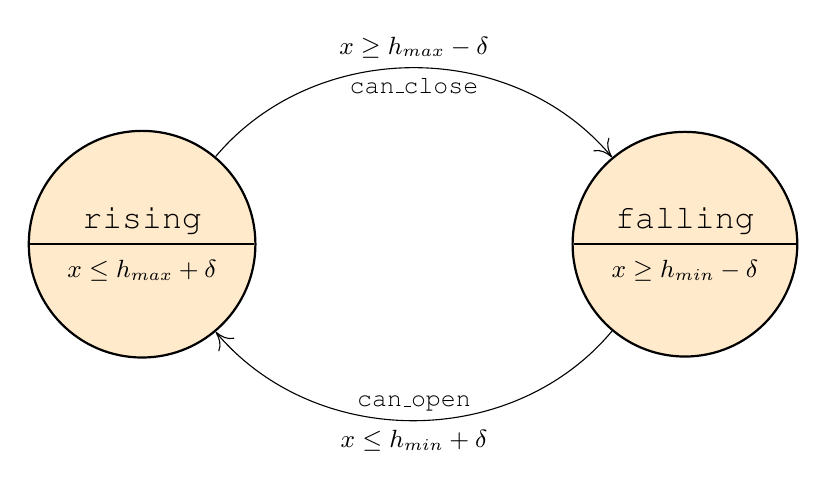
\begin{tikzpicture}
   \node[circle split, draw, thick, fill=lightorange] (rising)
   {\fontfamily{pcr}\selectfont \large rising \nodepart{lower} 
   \begin{tabular}{c}
   \small $x \leq h_{max}+\delta$
   \end{tabular} 
   };
   \node[circle split, draw, thick, fill=lightorange] (falling) [right=4 cm of rising] 
   {\fontfamily{pcr}\selectfont \large falling \nodepart{lower} 
   \begin{tabular}{c}
   \small $x \geq h_{min}-\delta$
   \end{tabular} 
   };
    \path[-{>[scale=2.5, width=3]},line width=0.4pt]
     (rising) edge[bend left=50] 
       node[anchor=north,above]{\small $x \geq h_{max}-\delta$}
       node[anchor=south,below]{\fontfamily{pcr}\selectfont \small can\_close} (falling)                  
       
     (falling) edge[bend left=50]  
       node[anchor=south,below]{\small $x \leq h_{min}+\delta$}
       node[anchor=north,above]{\fontfamily{pcr}\selectfont \small can\_open} (rising)     
     ;
\end{tikzpicture}
\end{center}

	
\end{document}